

\tikzset{every picture/.style={line width=0.75pt}} %set default line width to 0.75pt

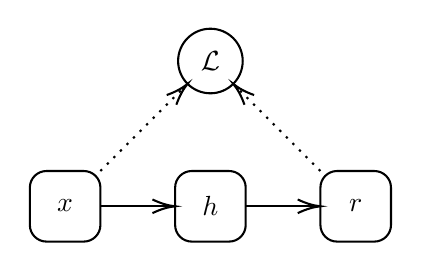
\begin{tikzpicture}[x=0.75pt,y=0.75pt,yscale=-1,xscale=1]
%uncomment if require: \path (0,148); %set diagram left start at 0, and has height of 148


% Text Node
\draw    (105, 28) circle [x radius= 15.56, y radius= 15.56]   ;
\draw (105,28) node   [align=left] {\begin{minipage}[lt]{13.735995849609345pt}\setlength\topsep{0pt}
\begin{center}
$\displaystyle \mathcal{L}$
\end{center}

\end{minipage}};
% Text Node
\draw    (88,89) .. controls (88,84.58) and (91.58,81) .. (96,81) -- (114,81) .. controls (118.42,81) and (122,84.58) .. (122,89) -- (122,107) .. controls (122,111.42) and (118.42,115) .. (114,115) -- (96,115) .. controls (91.58,115) and (88,111.42) .. (88,107) -- cycle  ;
\draw (105,98) node   [align=left] {\begin{minipage}[lt]{20.400000000000002pt}\setlength\topsep{0pt}
\begin{center}
$\displaystyle \boldsymbol{h}$
\end{center}

\end{minipage}};
% Text Node
\draw    (18,89) .. controls (18,84.58) and (21.58,81) .. (26,81) -- (44,81) .. controls (48.42,81) and (52,84.58) .. (52,89) -- (52,107) .. controls (52,111.42) and (48.42,115) .. (44,115) -- (26,115) .. controls (21.58,115) and (18,111.42) .. (18,107) -- cycle  ;
\draw (35,98) node   [align=left] {\begin{minipage}[lt]{20.400000000000002pt}\setlength\topsep{0pt}
\begin{center}
$\displaystyle \boldsymbol{x}$
\end{center}

\end{minipage}};
% Text Node
\draw    (158,89) .. controls (158,84.58) and (161.58,81) .. (166,81) -- (184,81) .. controls (188.42,81) and (192,84.58) .. (192,89) -- (192,107) .. controls (192,111.42) and (188.42,115) .. (184,115) -- (166,115) .. controls (161.58,115) and (158,111.42) .. (158,107) -- cycle  ;
\draw (175,98) node   [align=left] {\begin{minipage}[lt]{20.400000000000002pt}\setlength\topsep{0pt}
\begin{center}
$\displaystyle \boldsymbol{r}$
\end{center}

\end{minipage}};
% Connection
\draw  [dash pattern={on 0.84pt off 2.51pt}]  (52,81) -- (92.59,40.41) ;
\draw [shift={(94,39)}, rotate = 495] [color={rgb, 255:red, 0; green, 0; blue, 0 }  ][line width=0.75]    (10.93,-3.29) .. controls (6.95,-1.4) and (3.31,-0.3) .. (0,0) .. controls (3.31,0.3) and (6.95,1.4) .. (10.93,3.29)   ;
% Connection
\draw    (52,98) -- (86,98) ;
\draw [shift={(88,98)}, rotate = 180] [color={rgb, 255:red, 0; green, 0; blue, 0 }  ][line width=0.75]    (10.93,-3.29) .. controls (6.95,-1.4) and (3.31,-0.3) .. (0,0) .. controls (3.31,0.3) and (6.95,1.4) .. (10.93,3.29)   ;
% Connection
\draw    (122,98) -- (156,98) ;
\draw [shift={(158,98)}, rotate = 180] [color={rgb, 255:red, 0; green, 0; blue, 0 }  ][line width=0.75]    (10.93,-3.29) .. controls (6.95,-1.4) and (3.31,-0.3) .. (0,0) .. controls (3.31,0.3) and (6.95,1.4) .. (10.93,3.29)   ;
% Connection
\draw  [dash pattern={on 0.84pt off 2.51pt}]  (158,81) -- (117.41,40.41) ;
\draw [shift={(116,39)}, rotate = 405] [color={rgb, 255:red, 0; green, 0; blue, 0 }  ][line width=0.75]    (10.93,-3.29) .. controls (6.95,-1.4) and (3.31,-0.3) .. (0,0) .. controls (3.31,0.3) and (6.95,1.4) .. (10.93,3.29)   ;

\end{tikzpicture}